% !TEX encoding = ISO-8859-1

%% Material derivado de:
%% abntex2-modelo-include-comandos.tex, v-1.4 laurocesar
%% Copyright 2012-2013 by abnTeX2 group at http://abntex2.googlecode.com/ 
%%
%% This work may be distributed and/or modified under the
%% conditions of the LaTeX Project Public License, either version 1.3
%% of this license or (at your option) any later version.
%% The latest version of this license is in
%%   http://www.latex-project.org/lppl.txt
%% and version 1.3 or later is part of all distributions of LaTeX
%% version 2005/12/01 or later.
%%

% ---
% Este capítulo, utilizado por diferentes exemplos do abnTeX2, ilustra o uso de
% comandos do abnTeX2 e de LaTeX.
% ---
 
\chapter{Uso de nada do \protect{\LaTeX} e da classe abn\protect{\TeX}2}
\label{cap_exemplos}

%\chapterprecishere{Isto é uma sinopse de capítulo. A ABNT não 
%normatiza esse tipo de resumo, que não deve ser usado
%numa tese.  Use o comando 
%\emph{\texttt{\textbackslash{}chapterprecishere\{...\}}} para inserir a
%sinopse num documento.
%}\index{sinopse de capítulo}


É perfeitamente possível e, quiçá, até melhor, escrever uma 
tese ou dissertação sem usar nenhum dos comandos e ambientes 
da classe {abn\TeX{}2}, com exceção daqueles do pacote 
\texttt{abntex2cite.sty}, como \verb|\citeonline{..}|. 
Este capítulo mostra como usar alguns dos comandos do \LaTeX\ e 
comandos específicos da classe {abn\TeX{}2} que podem ser úteis na
preparação do seu documento. 

% ---
\section{Citações diretas e aforismos}
% ---

\index{citações!diretas}A classe {abn\TeX{}2} define o ambiente \texttt{citacao} para incluir
citações diretas com mais de três linhas, conforme normatizado na NBR10520 \cite{NBR10520:2002}:
\begin{citacao}
As citações diretas, com mais de três linhas, são
destacadas com recuo de 4 cm da margem esquerda, com letra menor que a do texto
e sem as aspas. Em documentos datilografados, deve-se
observar apenas o recuo (só a ABNT ainda usa máquina de escrever!) \cite[5.3]{NBR10520:2002}. 
\end{citacao}
O resultado é, sem sombra de dúvida, um insulto à tipografia de qualidade 
-- veja, por exemplo \citeonline[p.~17--18, 41]{bring04}.
Por isso, procure usar o ambiente do \LaTeX\ \texttt{quotation} para citações longas
e \texttt{quote} para aforismos e frases curtas. Nenhuma pessoa de sã
consciência vai se lembrar da NBR10520, de qualquer forma.   
Veja como uma citação fica muito melhor usando o ambiente \texttt{quotation}:
	\begin{quotation}\itshape
	As citações diretas com o ambiente \texttt{quotation} são
	destacadas com recuo de ambas as margens. 
	Se desejar usar letra menor que a do texto,
	utilize o comando \upshape{\verb|\small|}\itshape, logo após \upshape\verb|\begin{quotation}| \cite[p.~26]{LaTeX}.
	\end{quotation}

Citações curta podem aparecer entre aspas: ``A diferença entre a galinha e o político é 
que o político cacareja e não bota o ovo.'' (Millor Fernandes). Ou usando o ambiente \verb|quote|:
	\begin{quote}
	A diferença entre a galinha e o político é que 
	o político cacareja e não bota o ovo.
	\emph{Millor Fernandes}
	\end{quote} 

% ---
\section{Remissões internas}
% ---

Quando se faz referência no texto à Tabela~\ref{tab-aderencia}, têm-se um exemplo de remissão interna,
que também pode ser feita quando indicamos o \autoref{cap_exemplos}\footnote{O
número do capítulo indicado é
\ref{cap_exemplos}, que se inicia à página \pageref{cap_exemplos}.}
(\nameref{cap_exemplos}, \autopageref{cap_exemplos}), por exemplo.

Remissões internas ajudam o leitor a encontrar informação na tese. Notas de 
rodapé, por sua vez, confundem mais do que ajudam e dão a impressão de que você
se esqueceu de incluir algo no texto e, ao relê-lo, ficou com 
preguiça de reescrever todo o parágrafo e resolveu ``colar'' aquela informação
no rodapé da página. Por isso, evite a todo custo usar notas de rodapé.

% ---
\section{Tabelas}
% ---

\index{tabelas}A Tabela~\ref{tab-aderencia} é um exemplo de tabela construída em
\LaTeX, usando-se o pacote \verb|booktabs.sty|. Para aprender a usá-lo melhor, refira-se à documentação disponível no CTAN. 

Note que o \LaTeX\ posiciona os \emph{floats} 
(figuras ou tabelas) no topo ou no pé da página, porque esses elementos devem ``flutuar''
no documento e serem posicionados em locais convenientes \cite[p.~59]{LaTeX}. Com isso, costumam
ser colocados no topo (ou pé) da página seguinte à em que são mencionados pela 
primeira vez no texto. 

Pode-se usar uma outra família de fontes, como a sem serifa, para distinguir melhor a tabela
do texto do documento. Para fazer isso, inclua o comando \verb|\sffamily| antes de qualquer
texto da tabela (isso não altera o texto que aparece na lista de tabelas, que vai 
ser composto usando tipos com serifa).  A Tabela~\ref{tab-aderencia-rm} permite que você
compare os dois estilos e escolha o que mais lhe agradar.

As Tabelas~\ref{tab-aderencia} e \ref{tab-aderencia-rm} também ilustram o uso 
do ambiente \verb|minipage| para colocar duas ou mais tabelas ou figuras dentro
de um \emph{float}. Para aprender a fazer figuras e tabelas mais complexas,
consulte \emph{Using Imported Graphics in \protect{\LaTeX} and pdf\protect{\LaTeX}} \cite{epslatex06}, disponível no CTAN.

\begin{table}
\begin{minipage}[t]{72mm}\centering\sffamily
  {\caption[Valores da aderência $f$ para diversos estados do trilho] 
  		{Valores da aderência $f$ para diversos estados do trilho \cite{hay82}\label{tab-aderencia}}}
	%\vspace{4pt}
    {\footnotesize % usado para deixar as letras da tabela do mesmo tamanho das letras do caption
\begin{tabular}{ll} \toprule
  \textbf{\textit{Estado do trilho}} & \textbf{\textit{Aderência}} $f$ \\ \midrule
  Totalmente seco e limpo & 0,33 \\
  Lavado pela chuva       & 0,33 \\
  Seco e limpo            & 0,22 \\
  Seco e sujo             & 0,20 \\
  Úmido de orvalho        & 0,125 \\
  Úmido e sujo            & 0,11 \\
  Sujo com óleo           & 0,10 \\ \bottomrule
\end{tabular}}
\end{minipage}
\hfill
\begin{minipage}[t]{75mm}\centering\rmfamily
  \caption{Mesma tabela, com a mesma letra do texto \label{tab-aderencia-rm}}
	%\vspace{4pt}
    {\footnotesize % usado para deixar as letras da tabela do mesmo tamanho das letras do caption
\begin{tabular}{ll} \toprule
  \textbf{\textit{Estado do trilho}} & \textbf{\textit{Aderência}} $f$ \\ \midrule
  Totalmente seco e limpo & 0,33 \\
  Lavado pela chuva       & 0,33 \\
  Seco e limpo            & 0,22 \\
  Seco e sujo             & 0,20 \\
  Úmido de orvalho        & 0,125 \\
  Úmido e sujo            & 0,11 \\
  Sujo com óleo           & 0,10 \\ \bottomrule
\end{tabular}}
\end{minipage}
\end{table}


% ---
\section{Equações e expressões matemáticas}
% ---

\index{expressões matemáticas}Use o ambiente \texttt{equation} para escrever
equações  numeradas:
\begin{equation}
  x = \frac{-b \pm \sqrt{b^2-4ac}}{2a}.
\end{equation}
Também é possível usar colchetes para escrever uma expressão
matemática que não é numerada:
\[
\left|\sum_{i=1}^n a_ib_i\right|
\le
\left(\sum_{i=1}^n a_i^2\right)^{1/2}
\sqrt{\sum_{i=1}^n b_i^2}
\]

Às vezes, é preciso definir as variáveis e parâmetros de uma equação, 
como:
    \begin{equation}
    R_{r} = ( c_{1} + c_{2} \, V) \, G,
    \label{e3:3}
    \end{equation}
\begin{tabbing}
   em que \hspace{1em}
   \=$R_{r}$:  \hspace{2.3em}  \=resistência de rolamento [N] \\
   \>$V$:   \> velocidade do veículo [km/h]; \\
   \>$G$:   \> peso do veículo [kN]; e \\
   \>$c_1$ e $c_2$: \> constantes.
\end{tabbing}
Para isso, use o ambiente \texttt{tabbing}. Consulte o arquivo
usado para gerar o texto deste capítulo para um exemplo. Acima de 
tudo, lembre-se de que \emph{onde} só deve ser usado para se 
referir a locais geográficos; use \emph{em que}, \emph{na qual} etc.
para se referir à \autoref{e3:3}.

Numa linha de comando de texto, expressões matemáticas são colocadas en
\verb|$...$|, como em $ \lim_{x \to \infty} e^{-x} = 0 $, para que 
fiquem na mesma linha. Note que as variáveis numa
equação \emph{sempre} aparecem em itálico, mas números e funções matemáticas,
não. Além disso, não use itálico para escrever variáveis
no texto (e vice-versa), pois há diferenças visíveis entre o espaçamento 
no modo matemático (\verb|$...$|) e no itálico (\verb|\emph{...}|), além
do uso correto dos símbolos e sinais matemáticos. 
Use \verb|$y = x-1$| para escrever $y = x-1$ no texto,
ao invés de \emph{y = x-1}, obtido usando-se \verb|\emph{y = x-1}|.

Consulte um manual do \LaTeX\ para mais informações sobre como
escrever corretamente expressões matemáticas -- afinal de contas,
Donald Knuth criou o \TeX\ para tipografar matemática corretamente
\cite[p.~xiii]{LaTeX}.

\section{Figuras}

\index{figuras}Apesar de ser possível criar figuras diretamente em \LaTeX,
como o exemplo da \autoref{fig_circulo}, você certamente não vai querer 
fazer isso. O processo é insanamente tedioso e requer a entrada das
coordenadas $(x,y)$ iniciais e outras informações de todos as linhas
do gráfico.  

\begin{figure}
	\begin{center}
	    \setlength{\unitlength}{4cm}
		\begin{picture}(2,1)\thicklines
		\put(0,0){\vector(0,1){1}}
		\put(0,0){\vector(1,0){2}}
		\put(1.85,-.1){\footnotesize\emph{x}}
		\put(-.1,.85){\footnotesize\emph{y}}
		\linethickness{0.5mm}
		\qbezier(0,0)(0.5,0)(1,.5)
		\qbezier(1,0.5)(1.25,.9)(1.8,0.9)
		\end{picture}
	\end{center}
	\caption{Um gráfico desenhado com comandos do \protect{\LaTeX}}
	\label{fig_circulo}
\end{figure}
\begin{figure}\sffamily
	\begin{center}
	    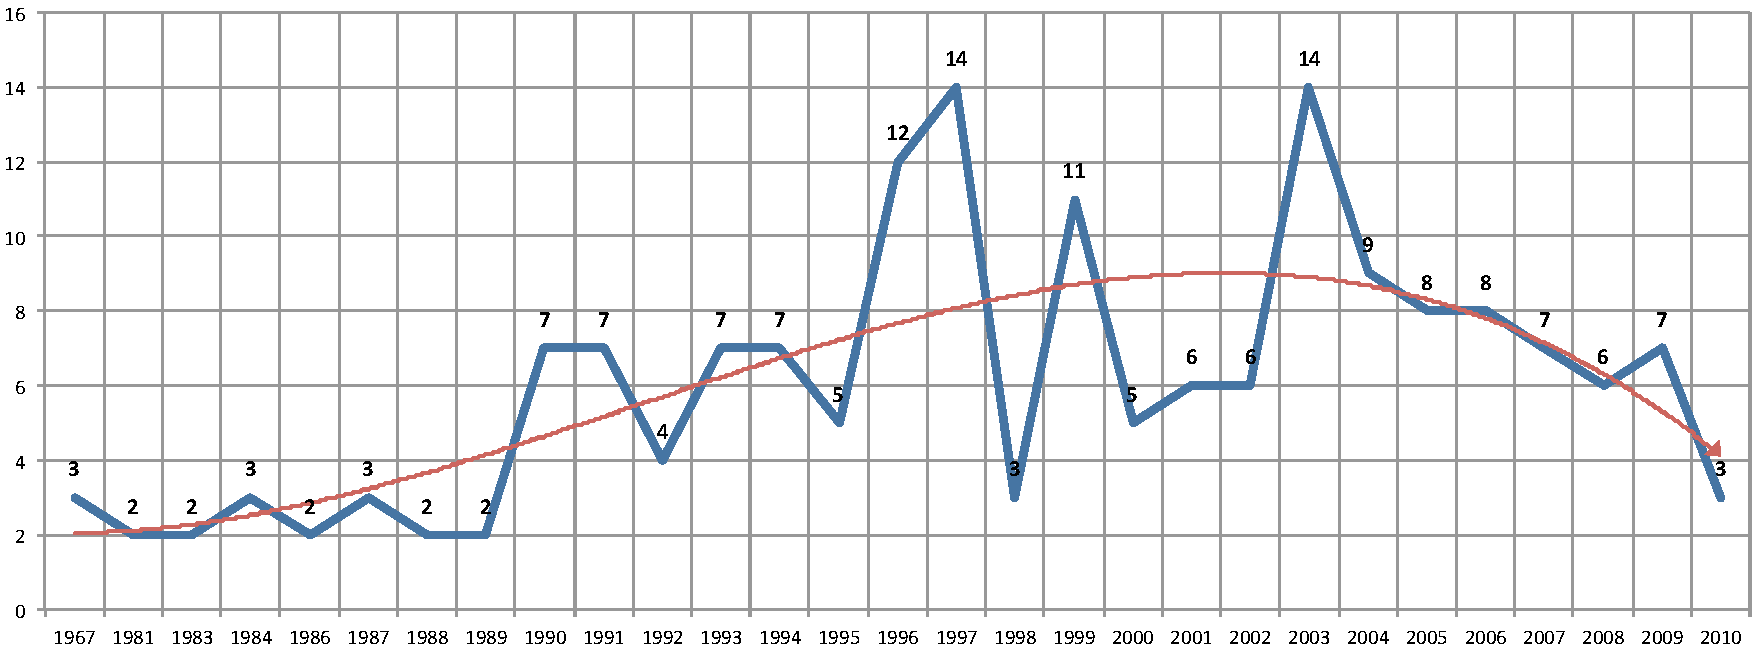
\includegraphics[width=160mm]{cap1/abntex2-img-grafico.pdf}
	\end{center}
	\caption[Gráficos feitos em Excel devem ser gravados como PDF para serem
	usados em \protect{\LaTeX}...]
	{Gráficos feitos em Excel devem ser gravados como PDF para serem
	usados em \protect{\LaTeX}, desde que o texto tenha uma tamanho legível
	quando reduzido para caber na página}
	\label{fig_grafico}
\end{figure}

É muito mais fácil incluir figuras usando arquivos externos, criados com
software dedicado (CorelDraw, Adobe Ilustrator, Inkscape etc.) ou, se 
for o caso de gráficos, com o MS-Excel ou OpenOffice Calc, entre outros. 
A referência básica para inclusão de figuras usando arquivos externos é
\emph{Using Imported Graphics in \protect{\LaTeX} and pdf\protect{\LaTeX}} 
\cite{epslatex06}, disponível no CTAN.tug.org 
\href{ftp://ctan.tug.org/tex-archive/info/epslatex.pdf}{\fbox{\texttt{link}}}. 
Vale a pena consultar, porque há
exemplos para todos os casos possíveis e imagináveis.



\begin{figure}\sffamily
	\begin{center}
	    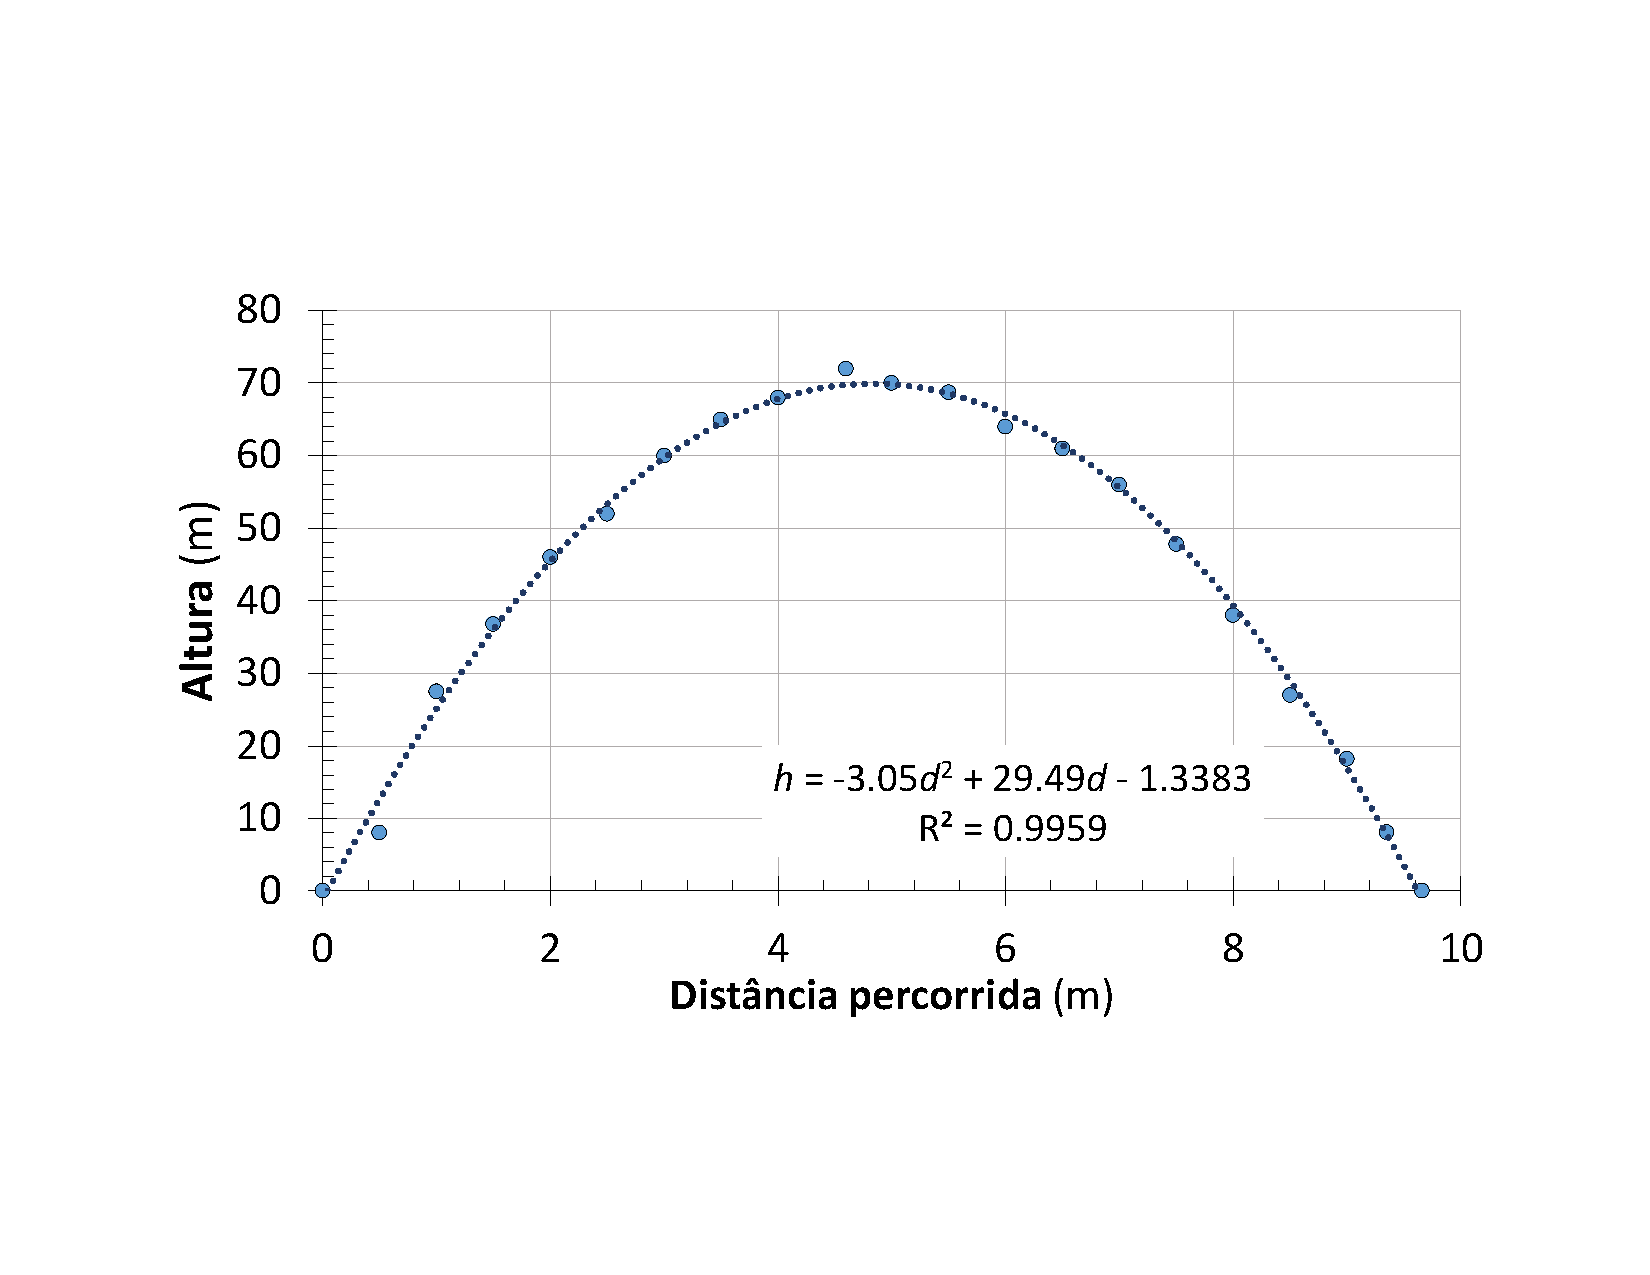
\includegraphics[height=60mm]{cap1/grafico1b.pdf}
	\end{center}
	\vspace{-12pt} % reduz espaço entre figura e caption
	\caption{Gráfico preparado com maior cuidado, incluindo títulos dos eixos
	e unidades}
	\label{fig_grafico1b}
%\end{figure}
%\begin{figure}\sffamily
	\centering
	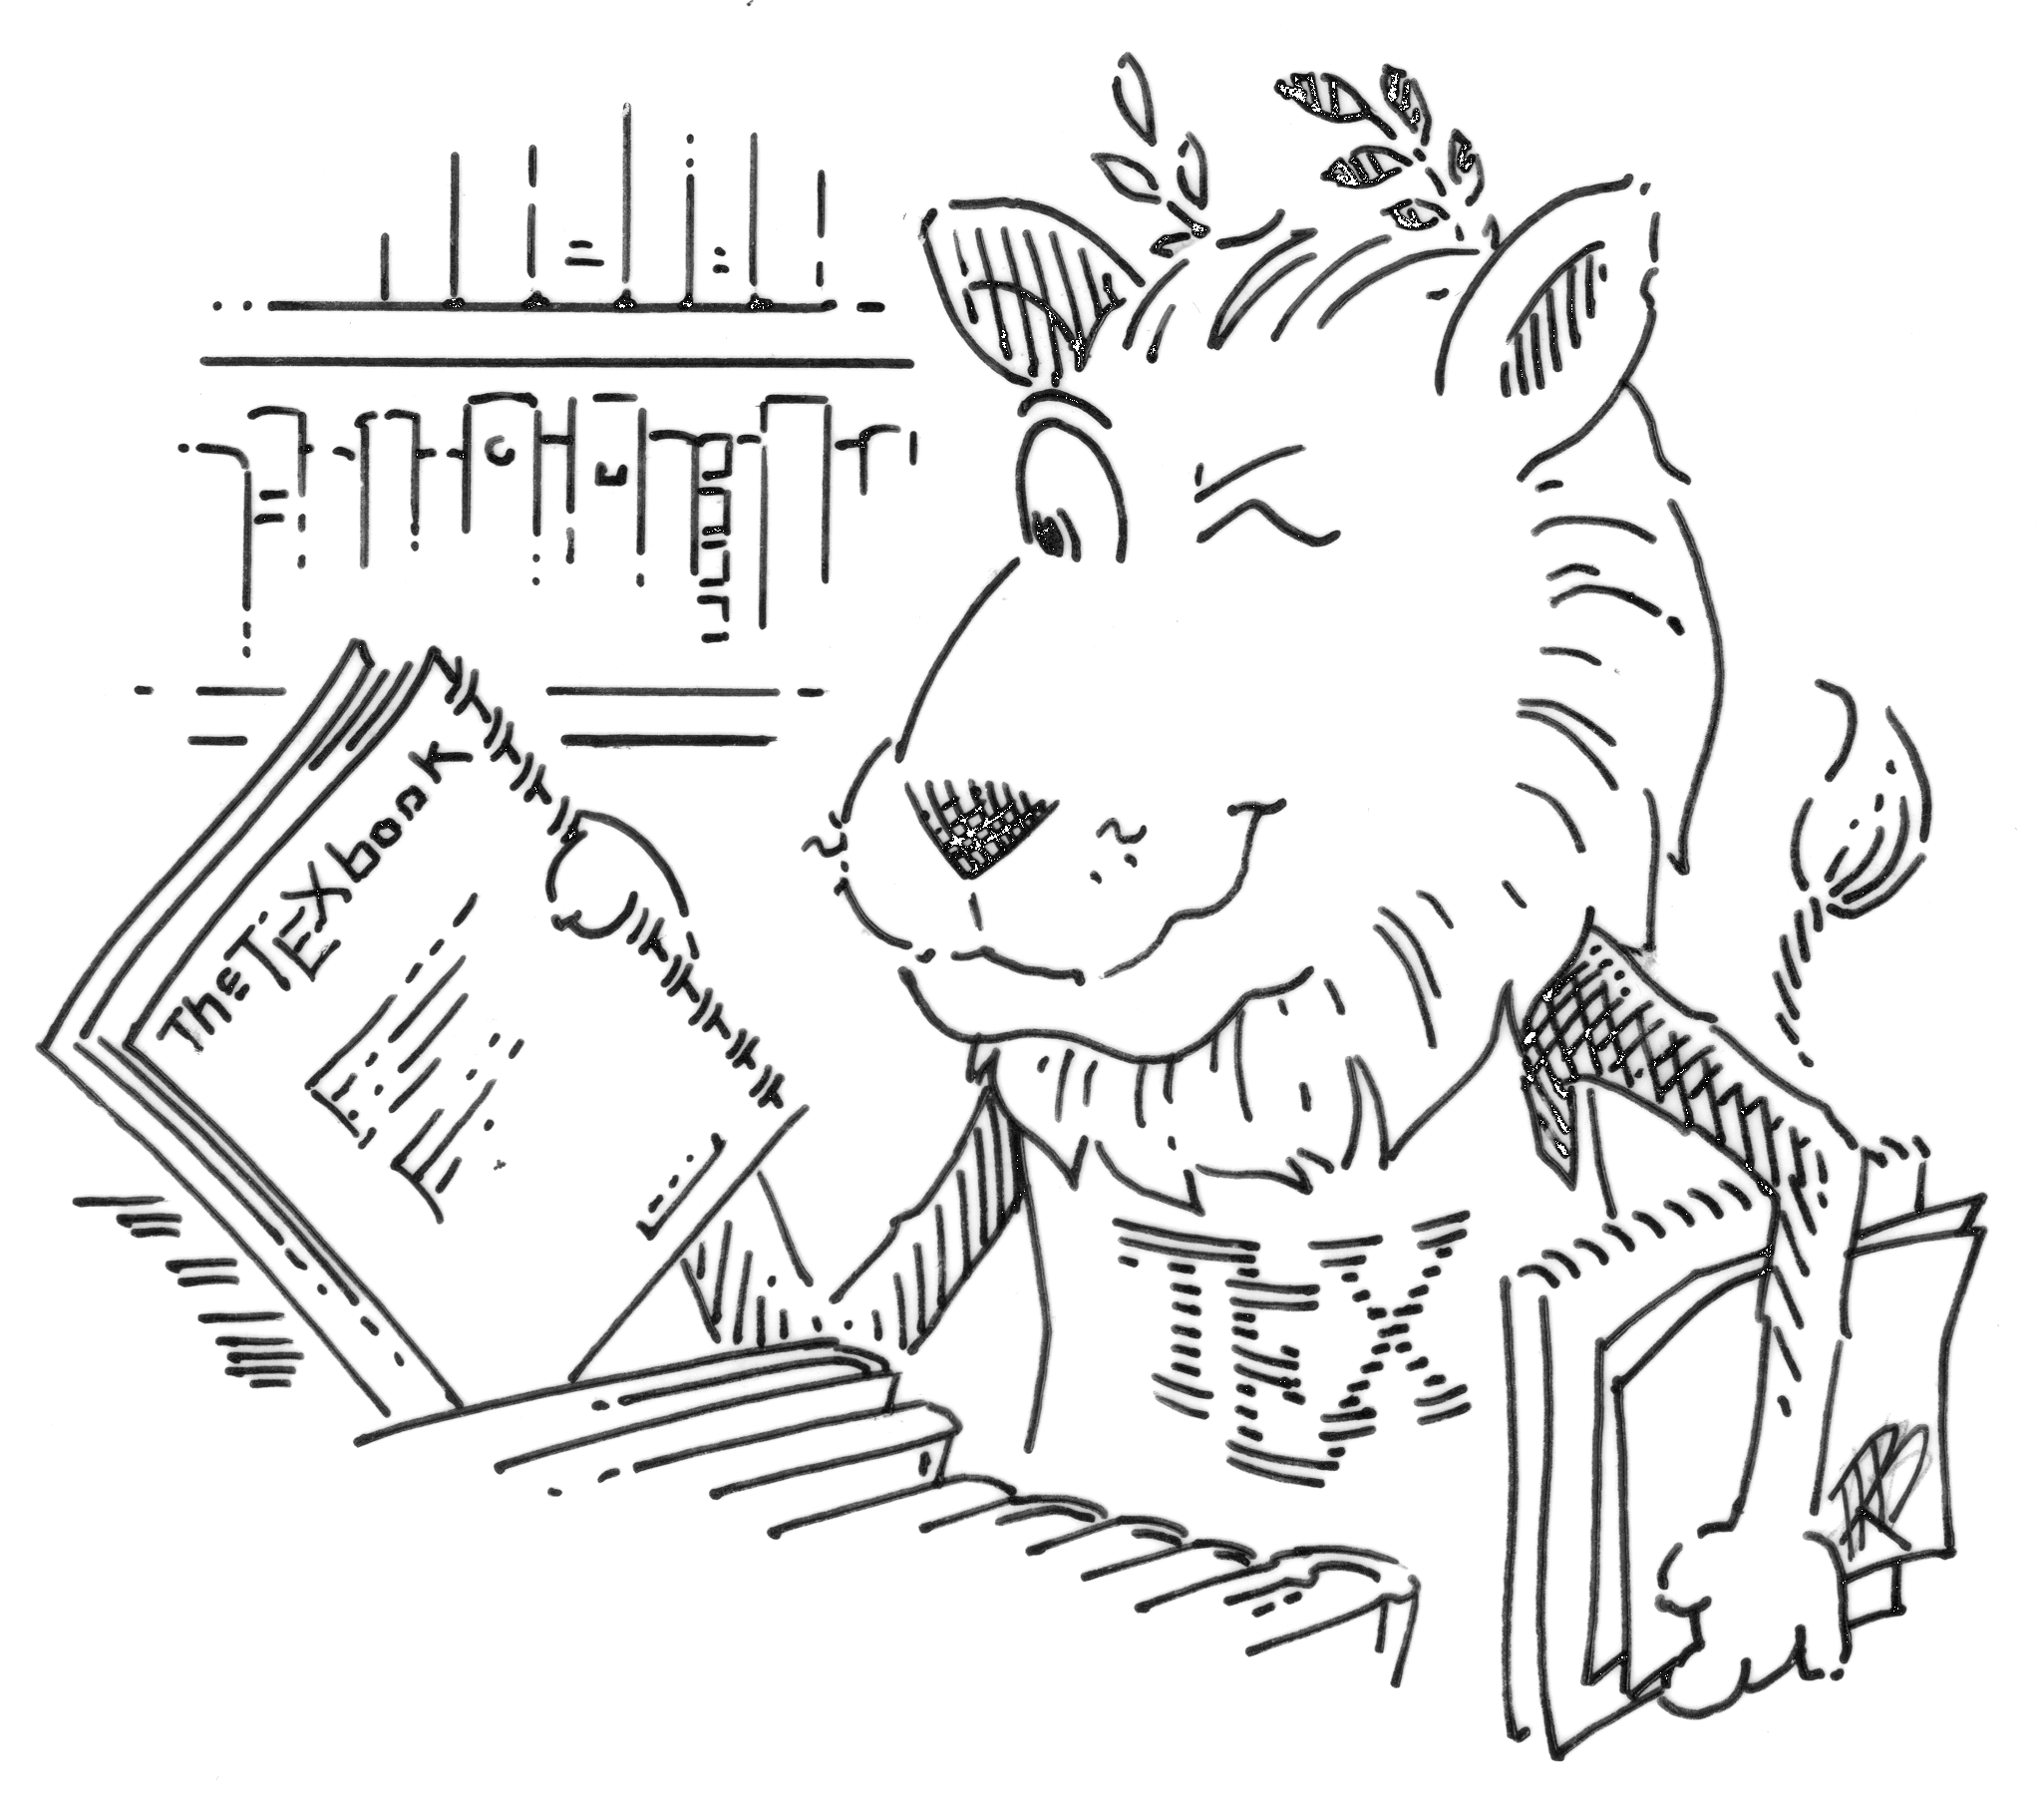
\includegraphics[height=60mm]{cap1/tex_lion_600.png}
	\caption{Arquivos raster do tipo JPEG ou PNG podem
	ser incluido diretamente em figuras}
	\label{f:lion}
\end{figure}



Na \autoref{fig_grafico}, \texttt{abntex2-img-grafico.pdf}  é um  arquivo 
externo, usado no ambiente \texttt{figure}. O gráfico foi elaborado no Excel
e pode-se notar que há um problema com o tamanho das letras, que ficaram
praticamente ilegíveis quando a figura foi reduzida para a largura da página,
160~mm. Com um certo cuidado, é possível criar uma figura bem mais legível, 
como pode visto na \autoref{fig_grafico1b}. 

O ideal é que as letras e números
na figura combinem em aparência com as usadas no texto. Se você 
optar por usar caracteres sem serifa nas tabelas, faça isso para todas elas
e use também os mesmos caracteres sem serifa nas figuras. Procure fazer
com que os caracteres das figuras sejam 10--20\% menores que o do texto, 
lembrando-se de que poderão ser reduzidos para caber na página. Planejando
o tamanho da figura no texto (por ex., 160~mm de largura), é possível escolher
o tamanho dos caracteres no Excel. Na  \autoref{fig_grafico1b}, o tamanho 
original dos caracteres é 12~pt e as dimensões do gráfico gerado pelo Excel são 
$228 \times 126$~mm, com números de 5~mm de altura.


A vantagem de usar imagens vetoriais (como o arquivo \texttt{grafico1b.pdf}) é
que, não importa a escala escolhida (opção \texttt{[width=100mm]}), as figuras
sempre aparecerão com a máxima qualidade. Além disso, os arquivo final do 
texto ficará menor. No entanto, o \LaTeX\ também permite a inclusão de arquivos
raster do tipo \textsc{jpeg} ou  \textsc{png}. A \autoref{f:lion} exemplifica como
inserir um arquivo raster numa figura em \LaTeX\ usando o comando \texttt{%
\textbackslash{}includegraphics[\textrm{\emph{opt}}]\{\textrm{\emph{arq}}\}}.


% ---
\section{Enumerações: comandos do \LaTeX\ e do {abn\TeX{}2}}
% ---

Para a criação de listas, a classe \abnTeX\ fornece os 
ambientes \texttt{alineas}, \texttt{subalineas} e \texttt{incisos}, 
que complementam os ambientes \texttt{itemize}, \texttt{enumerate}
e \texttt{description} do \LaTeX. 

\index{alíneas}\index{subalíneas}\index{incisos} A NBR6024 
 determina que a organização
de assuntos de uma seção que não possuam títulos deve ser
feita através de alíneas \cite[item~4.2]{NBR6024:2012}:

\begin{alineas}
  \item os diversos assuntos que não possuam título próprio, dentro de uma mesma
  seção, devem ser subdivididos em alíneas\footnote{As notas de rodapé devem ficar
  dentro das margens, separadas do texto por um espaço simples entre as
  linhas e por filete de 5 cm, a partir da margem esquerda. Devem ser
  alinhadas, a partir da segunda linha da mesma nota, abaixo da primeira letra
  da primeira palavra, de forma a destacar o expoente, sem espaço entre elas e
  com fonte menor. \citeonline[5.2.1]{NBR14724:2011}}; 
  
  \item o texto que antecede as alíneas termina em dois pontos;
  \item as alíneas devem ser indicadas alfabeticamente, em letra minúscula,
  seguida de parêntese. Utilizam-se letras dobradas, quando esgotadas as
  letras do alfabeto;

  \item as letras indicativas das alíneas devem apresentar recuo em relação à
  margem esquerda;

  \item o texto da alínea deve começar por letra minúscula e terminar em
  ponto-e-vírgula, exceto a última alínea que termina em ponto final;

  \item o texto da alínea deve terminar em dois pontos, se houver subalínea;

  \item a segunda e as seguintes linhas do texto da alínea começa sob a
  primeira letra do texto da própria alínea;
  
  \item subalíneas  são um segundo nível 
  do ambiente \texttt{alineas} e  devem ser conforme as alíneas a
  seguir \cite[item~4.3]{NBR6024:2012}:

  \begin{alineas}
     \item as subalíneas devem começar por travessão seguido de espaço;

     \item as subalíneas devem apresentar recuo em relação à alínea;

     \item o texto da subalínea deve começar por letra minúscula e terminar em
     ponto-e-vírgula. A última subalínea deve terminar em ponto final, se não
     houver alínea subsequente;

     \item a segunda e as seguintes linhas do texto da subalínea começam sob a
     primeira letra do texto da própria subalínea;
     
     \item a classe \abnTeX\ só permite dois níveis do ambiente 
     \texttt{alineas}. 
     
%     \item O terceiro nível deve ser feito com o ambiente
%     \texttt{incisos} e a única diferenciação passa a ser o recuo,
%     pois todos os itens usam o travessão:
%     
%       \begin{incisos}
%    		\item um novo inciso;
%%    		\item mais um nível pode ser criado usando o ambiente 
%%    		\texttt{subalineas}:
%%			  \begin{subalineas}
%%			    \item uma subalínea dentro de um inciso;
%%			    \item uma subalínea usada como um segundo
%%			    nível de \texttt{incisos} (veja o código); 
%%			  \end{subalineas}
%  		\end{incisos}

  \end{alineas}
  
  \item no \abnTeX\ estão disponíveis os ambientes \texttt{incisos} e
  \texttt{subalineas} que, em suma, são o mesmo que se criar outro nível de
  \texttt{alineas}, como nos exemplos à seguir (veja o código):
  
  \begin{incisos}
    \item \textit{um novo inciso em itálico};
    \item ou um inciso sem itálico, que o faz igual a uma subalínea que,
    por sua vez, é um ambiente \texttt{subalineas} dentro de um outro
    \texttt{subalineas};
  \end{incisos}
    
  \item Última alínea com \emph{ênfase}.
  
\end{alineas}

Resumindo, é melhor usar apenas o ambiente \texttt{alineas} quando for
preciso fazer uma lista numerada alfabeticamente; se for preciso fazer
uma sublista dentro desta lista, use \texttt{incisos} ou \texttt{subalineas}
se quiser que ela tenha travessão.

É também possível combinar \texttt{alineas} com \texttt{enumerate} e/ou
\texttt{itemize}, para maior clareza:
  \begin{alineas}
    \item neste caso, \texttt{alineas} faz com o primeiro nível seja enumerado
    	com letras;
    	\begin{enumerate}
    		\item o segundo nível, criado com \texttt{enumerate}, enumera as 
    		alíneas numericamente;
    	\begin{itemize}
    			\item o terceiro nível pode ser criado com \texttt{itemize};
    			\item as alíneas do terceiro nível iniciam-se com um símbolo.
    			\begin{itemize}
    			\item um quarto nível pode ser necessário em alguns casos;
	    			\begin{itemize}
	    			\item um quinto nível pode ser demais;
		    			\begin{itemize}
		    			\item um sexto nível é brincadeira;
		    			\end{itemize} 
	    			\end{itemize} 
    			\end{itemize} 
    		\end{itemize}
    		\item as alíneas do segundo nível começam com um número;
    	\end{enumerate}
    \item uma alínea do primeiro nível inicia-se com uma letra (veja o código); e
    \item a ordem de uso dos ambientes \texttt{alineas}, \texttt{enumerate} e
    \texttt{itemize} pode ser modificada da forma que for mais conveniente para
    a clareza do texto.
  \end{alineas}
Outra forma de organizar as listas poderia ser variando a sequência de ambientes
de lista:
  \begin{enumerate}
    \item neste caso, \texttt{enumerate} faz com o primeiro nível seja enumerado
    	numéricamente;
    	\begin{alineas}
    		\item o segundo nível, criado com \texttt{alineas}, enumera as 
    		alíneas com letras;
    		\begin{incisos}
    			\item o terceiro nível pode ser criado com \texttt{incisos};
    			\item as alíneas do terceiro nível iniciam-se com um travessão. 
    		\end{incisos}
    		\item as alíneas do segundo nível começam com uma letra e parenteses;
    	\end{alineas}
    \item uma alínea do primeiro nível inicia-se com um número (veja o código); e
    \item a ordem de uso dos ambientes \texttt{alineas} e \texttt{enumerate} 
     foi ser modificada para aumentar a clareza do texto.
  \end{enumerate}

% ---
\section{Inclusão de outros arquivos}\label{sec-include}
% ---

É uma boa prática dividir o seu documento em diversos arquivos, e não
apenas escrever tudo em um único. Esse recurso foi utilizado neste
documento. Para incluir diferentes arquivos em um arquivo principal,
de modo que cada arquivo incluído fique em uma página diferente, utilize o
comando:

\begin{verbatim}
   \include{dir/arquivo-a-ser-incluido}      % sem a extensão .tex
\end{verbatim}

Para incluir documentos sem quebra de páginas, utilize:

\begin{verbatim}
   \input{dir/arquivo-a-ser-incluido}      % sem a extensão .tex
\end{verbatim}

% ---
\section{Compilar o documento \LaTeX}
% ---

Geralmente os editores \LaTeX, como o \TeX{}studio ou \TeX{}works
compilam os documentos automaticamente, de modo que você não precisa se
preocupar com isso.


